\section{Theories of Motivation}

There are many theories of how people learn, how to teach, and how to engage with students. 
In this proposal, I investigate Academic Motivation - the process by which people choose to direct energy towards learning.
Motivation is well understood to be a crucial part of education, particularly in Computer Science~\cite{Carter:2011}.

\subsection{MUSIC Model of Academic Motivation}

In this preliminary proposal, I lean on the MUSIC Model of Academic Motivation as a primary framework.
The decision to use the MUSIC model was based on several criteria.
Although there are many motivational models available, few strive to be holistic models specifically developed for academics.
For example, theories like Expectancy-Value and Cognitive Evaluation Theory have a wider scope and have stemmed from other disciplines such as healthcare. %TODO: Cite
The MUSIC Model is derived from a meta-analysis of these other theories, incorporating only the academically relevant components.
Further, the MUSIC model is a tool meant for both design and evaluation, allowing it to be used in all phases of this work.
Finally, the model and its associated instrument, the MUSIC Model of Academic Motivation Inventory (MMAMI) , has been extensively validated and utilized in other educational domains, making it a reliable device\cite{jones-validity}.

The MUSIC model identifies five key constructs in motivating students \cite{jones-description}:
\begin{description}
	\item[eMpowerment:] The amount of control that a student feels that they have over their learning -- e.g., course assignments, lecture topics, etc. This is amount of Agency that a student percieves.
	\item[Usefulness:] The expectation of the student that the material they are learning will be valuable to their short- and long- term goals. There is no clear delineation of the time-scale for these goals, but there is nonetheless a distinction between strategic skills that students need to be successful in careers and personal interests and the tactical skills they need to complete present-day tasks.
	\item[Success:] The student's belief in their own ability to complete assignments, projects, and other elements of a course with the investment of a reasonable, fulfilling amount of work. Most students desire experiences that are successful, but still challenging enough to be worth it.
	\item[Interest:] The student's perception of how the assignment appeals to situational or long-term, individual interests. The former covers the aspects of a course related to attention, while the latter covers topics related to the fully-identified areas of focuses of the student. It can be difficult to parse out the difference between individual interests and long-term career goals -- there can be alignment between these two components.
	\item[Caring:] The students perception of other stakeholders' attitudes toward them. These stakeholders primarily include their instructor and classmates, but also can be extended to consider other members of their learning experience (e.g., administration, external experts, etc.). It can also be viewed as the extension towards society as a whole.
\end{description}

Students are motivated when one or more of these constructs is sufficiently activated.
They are not all required to achieve maximal levels, and in fact that is not always desired -- it is possible, for instance, for a student to feel too empowered, and become overwhelmed by possibilities.
For some of these constructs, a careful balance is required, and it may not be possible to ever achieve a minimal level; no matter how exciting you make your lecture, you may never convince your students it is interesting, although it is possible that they will still consider it useful and stay motivated.
Crucially, students' subjective \textit{perception} of these constructs is a defining requirement and is more important than objective reality.
It does not matter if you believe that your lecture is Useful, if you have not convinced your students that it is (although an instructor's beliefs are a powerful tool for convincing their students).

The MUSIC model is often used as an organizational framework and an evaluative tool.
As the former, it is a list of factors to consider when building modules, assignments, and content of a course.
At all times, instructors can consider whether they are leveraging at least one construct to motivate their students.
As the latter, it offers both a quantified instrument (MMAMI) and a structure to anchor a qualitative investigation on.
The model has also directly been used tactically in course design: Jones describes a controlled classroom experiment to motivate students by having an experimental group reflect on how a course satisfies the constructs of the MUSIC model. Students were simply prompted to answer the question ``How will the material presented here will be useful to you?''.
Quantitative data gathered after the experiment indicated a significant increase in motivation~\cite{mcginley2014brief}.
The MUSIC model is therefore a very flexible resource for studying motivation.

The MUSIC model has not been seriously applied to Computer Science education before, although a number of other motivational frameworks have been leveraged in studies.
Many of these studies often find results that hint at many of the elements of the MUSIC model.
For instance, Mitchell~\cite{Mitchell:2000} interest, usefulness, and ``intellectual challenges'' (success) as three primary elements influencing success in computer science.
Although they do not discuss empowerment and social elements, many other studies often suggest these themes.
Still, it should be acknowledged that it is an open question whether the MUSIC model can be applied directly, or if this domain has different characteristics from other disciplines.

\subsection{Situated Learning Theory and Authenticity}

Although most of this proposal relies on the MUSIC Model of Academic Motivation, I will discuss Situated Learning Theory briefly.
Situated Learning Theory, originally proposed by Lave and Wenger, argues that learning normally occurs as a function of the activity, context, and culture in which it is situated~\cite{lave-situated}.
Therefore, tasks in the learning environment should parallel real-world tasks, in order to maximize the \textit{authenticity}.
Contextualization is key in these settings, as opposed to decontextualized (or ``inert'') settings.
The key difference is that learning is driven by the problem being solved, rather than the tools available – therefore, the problem being solved should lead directly to the tool being taught.
This argument suggests that this is a key aspect of motivating students.

Authenticity is a crucial, recurring theme within Situated Learning Theory.
All instruction and assessment must be aligned with reality such that success in the former leads to success in the latter.
However, there is a subtle nuance here -- authenticity is a perceived trait, not an objective one.
Students derive value from their learning only if they \textit{perceive} authenticity, regardless of whether the instructor has successfully authenticated the experience.

Situated Learning Theory has been applied to the domain of Computer Science before, with mixed results. A seminal paper by Ben-Ari \cite{ben2004situated} explores its application and limitations.
This paper is somewhat hasty in its application of SL Theory by taking a macro-level view -- they narrowly look to Open-Source and Industry Software Development communities as the only potential CoPs and interpret SL Theory as strictly requiring constant legitimacy, largely ignoring the possibility for gradual development of authenticity within individual courses and modules throughout a curriculum:

\begin{quote}
What I am claiming is that situated learning as presented in their work cannot be accepted at face value, because it simply ignores the enormous gap between the world of education and the world of high-tech CoPs, which demand extensive knowledge of both CS subjects and applications areas.
This gap can only be bridged by classical decontextualized teaching in high schools, colleges and universities.
\end{quote}

However, other researchers have found it a useful lens for analyzing curricula.
For instance, Guzdial and Tew \cite{guzdial2006imagineering} used the theory to innovatively explore and deal with the problem of inauthenticity within their Media Computation project.
SL Theory clearly has value, but only as a function of the way that it is applied.
In this preliminary proposal, I will take advantage of SL Theory as a generalized tool for exploring the topic of authenticity throughout introductory Computer Science.

The original work in Situated Learning Theory was categorically not about pedagogy or instructional design- it described how people learn and the importance of context and collaboration, but it did not recommend a particular style of classroom.
Subsequent research by Brown \cite{brown1989situated} and others expanded the theory so that it could be applied to the design of learning experiences.
These expansions often naturally dictate the use of active learning techniques, reducing the role of lecture in favor of collaborative, problem-based learning activities.
Choi \& Hannafin \cite{situated-cognition} describe a particularly useful, concrete framework for designing situated learning environments and experiences.
The Choi \& Hannafin framework has four key principles:

\begin{description}
	\item[Context] ``... The problem's physical and conceptual structure as well as the purpose of activity and the social milieu in which it is embedded''\cite{rogoff1984everyday}, context is driven not just by the atmosphere of the problem at hand, but also by the background and culture surrounding the problem.
	A good context enables a student to find recognizable elements and build on prior understanding, eventually being able to freely transfer their learning to new contexts.
	\item[Content] The information intending to be conveyed to the students.
	If context is the backdrop to the learning, then content might be seen as the plot.
	Naturally, context and content are deeply intertwined with each other, and its difficult to talk about one without referencing the other; in fact, content is an abstract entity that needs to be made concrete through contextualization when it is delivered to the learner.
	If the information is too abstract, than it will never connect with the learner and will not be transferable to new domain.
	However, if it is too grounded in a domain, then it will not be clear how it can be re-applied elsewhere. 
	Ultimately, content must be given in a variety of forms to maximize transfer.
	Two useful methods for building content are anchored instruction (exploring scenarios, or anchors, in the context based on the content) and cognitive apprenticeship (mediating knowledge from an expert to the novice learner in a mentoring relationship).
	\item[Facilitations] The modifications to the learning experience that support and accelerate learning.
	Facilitations provide opportunities for students to internalize what they are learning by lowering the barriers that can surround situated experiences, possibly at the cost of some amount of authenticity. 
	These modifications might be technological in nature, but they can also be pedagogical.
	Although there are many different forms that Facilitations can take, Scaffolding is one of the most common.
	Scaffolding is a form of support that is intended to extend what a learner can accomplish on their own.
	This support is required at the onset of the learning process, but is unnecessary once a sufficient threshold has been passed; during this transition, the amount of scaffolding can be tuned to the learners understanding.
	In Computer Science, for instance, students often take advantage of software libraries and frameworks to create sophisticated graphical programs that would be beyond daunting if implemented from scratch.
	\item[Assessment] The methods used to assess the learning experience and the progress of the student.
	Choi \& Hannafin gives special attention to the “teach to the test” problem, and how assessment needs to change to measure students' ability to solve authentic problem (as opposed to their ability to solve the test’s specific problem), and to be able to transfer their understanding when solving different but related problems.
	It is important that assessment is measured against the individualized goals and progress of a learner, requiring that any standards used be fluid and adaptable to different learners personal situations.
	Of course, assessment should be an on-going part of the learning process, providing feedback and diagnostics.
	Ultimately, the learner should join in the process of assessment as they transition to an expert – being able to meta-cognitively self-evaluate the effectiveness of ones methods and communicate results to others are key abilities of experts. 
\end{description}

\subsection{Contexts vs. Content}

\begin{wrapfigure}{R}{0.5\textwidth}
		\begin{center}
				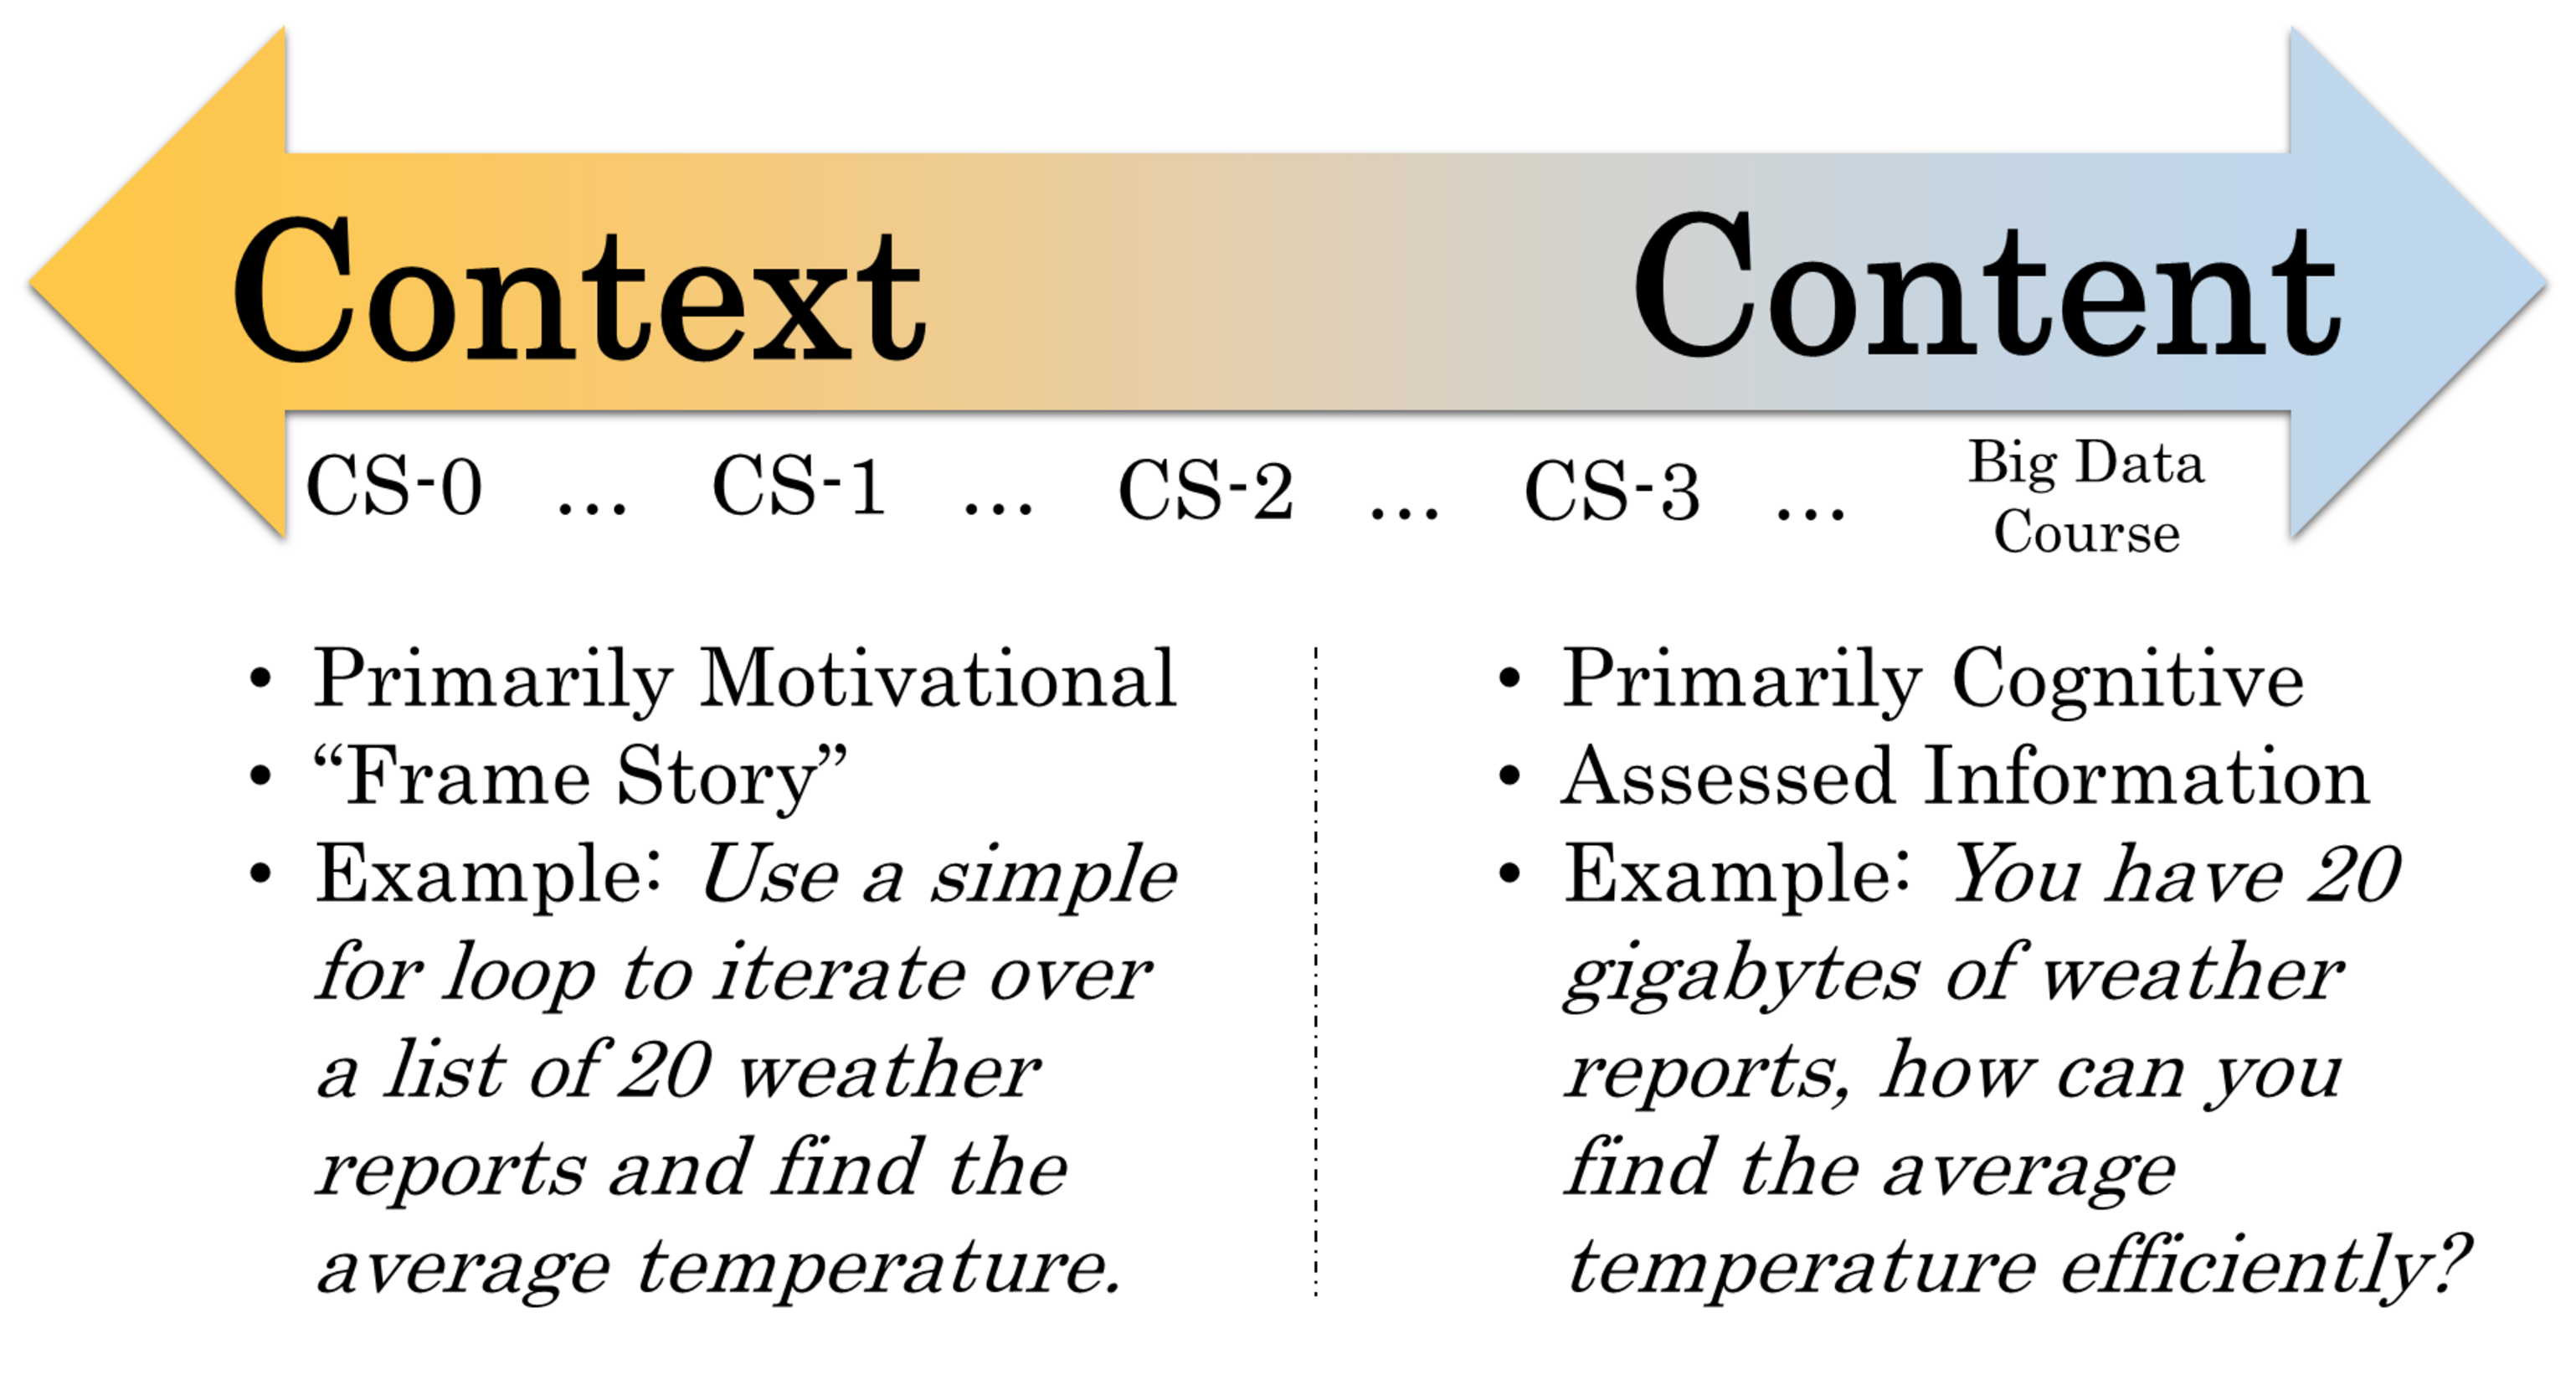
\psfig{file=images/content-context-2.eps, width=\linewidth}
		\end{center}
		\caption{Content vs. Context}
		\label{fig-content-context}
\end{wrapfigure}

There is a reciprocal relationship between contexts and content.
Figure \ref{fig-content-context} demonstrates an example of this relationship for the expected emphasis on big data as a context vs. content throughout an undergraduate curriculum, from a CS-0 (non-majors) course all the way to an upper-level course specifically on big data.
Just as the upper-level course would naturally use big data as its context and content, a CS-0 course could still have content related to big data.
However, the majority of the use of big data would be as the framing story for assignments, especially in earlier parts of the course.
When students learn programming in the context of, say, game development, they are almost necessarily learning content related to game development that may not be universal to computer science -- e.g., how graphical resources are organized and accessed within the game engine.
This content may be seen as a distraction by the instructor, or as useful side knowledge - for example, if a student had to learn how to use a command line in order to compile their game, they would be learning an authentic skill that might not be considered part of the core content, but is nonetheless generally useful.
When evaluating a context, it is useful to consider what content it represents, and how authentic and useful it is.
The authenticity of content that is attached to a context affects the authenticity of the learning environment as a whole.

Fascinatingly, the need for a strong context diminishes as learners mature and become domain-identified -- the content itself becomes the context.
Learners start to see other contexts as nothing more than distractions and unnecessary fluff.
This makes sense -- you would hope that Computer Science majors in their third semester would be naturally interested in the material, and this is borne out in experimental data.
For instance, Yarosh \& Guzdial attempted to integrate Media Computation in a CS-2 (Data Structures) course, and found that the learners had ``outgrown the desire for a context''~\cite{yarosh2008narrating}. 
These results are similar to results we found in our interventions with a CS-3 (Data Structures and Algorithms), where students seemed more irked by the surrounding context than intrigued.


\begin{figure}[!ht]
	\begin{center}
		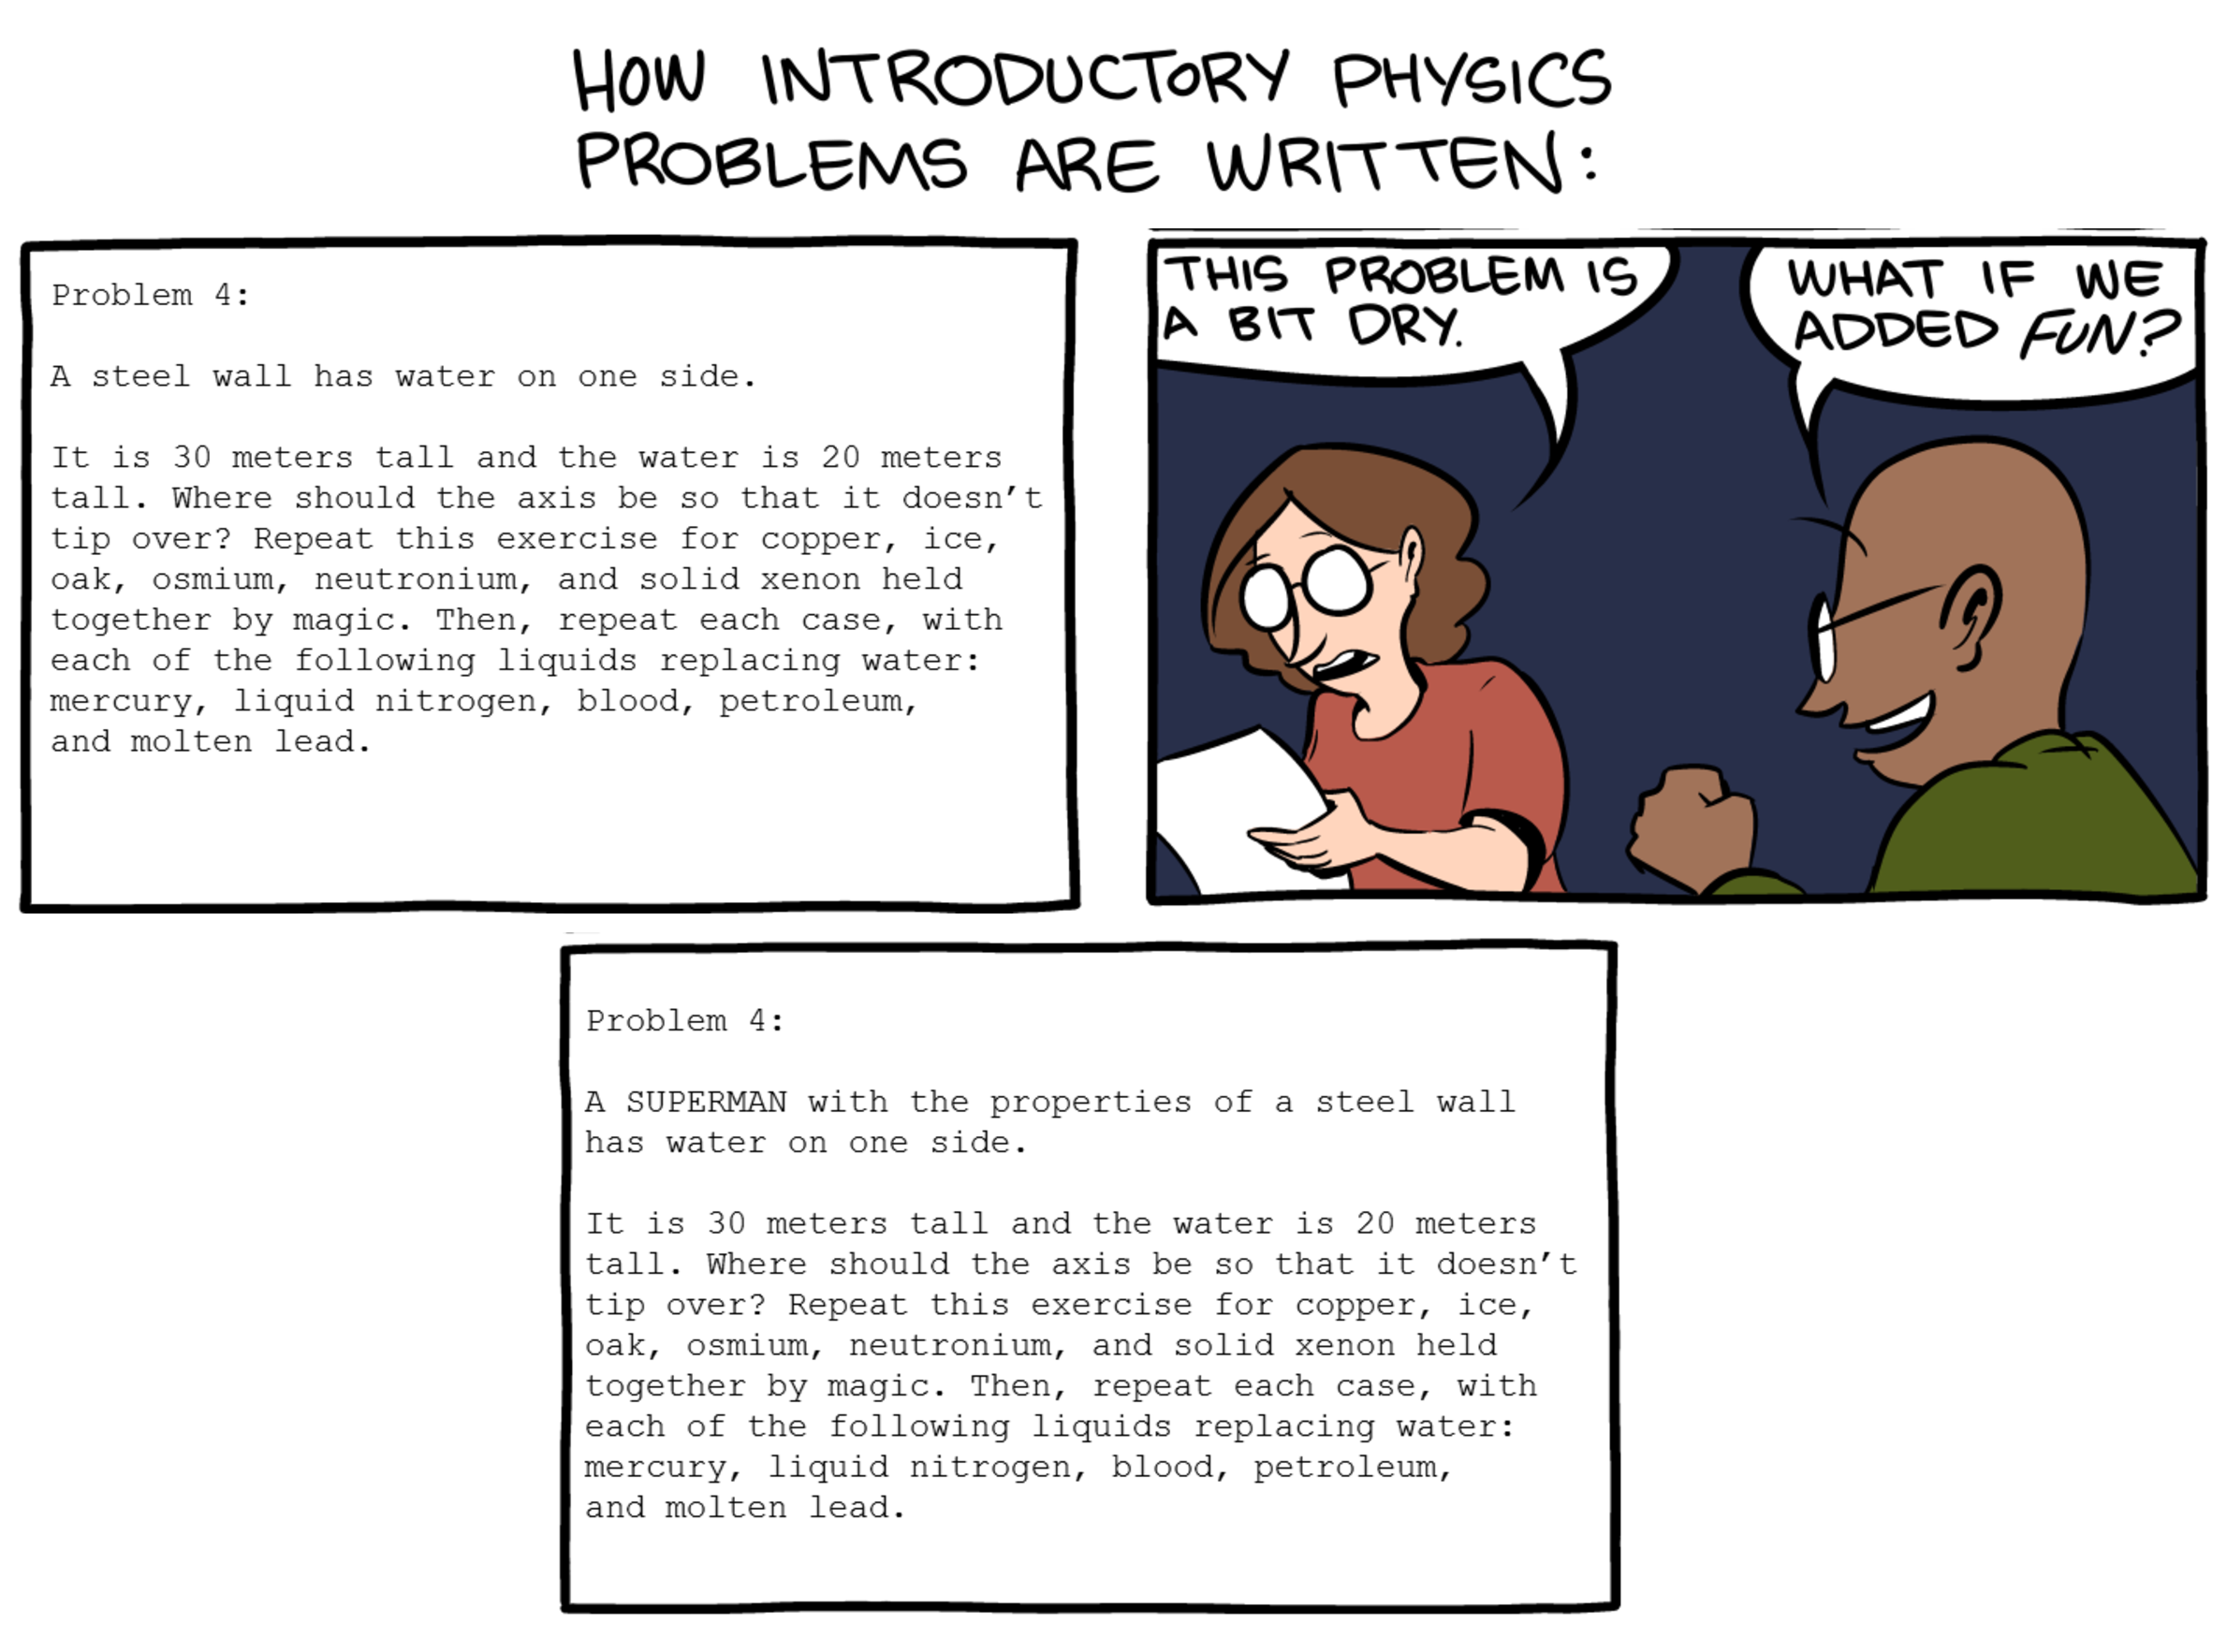
\psfig{file=images/smbc.eps, width=\linewidth}
	\end{center}
	\caption{How to Add Fun to Education}
	\textit{Making the context ``Fun'' is not necessarily trivial, whether in physics education or computer science education.~\cite{SMBC}}
	\label{fig-comic-context}
\end{figure}

Of course, it is up to instructor to determine the depth and breadth of the context's integration.
The trade-off between the value and distraction added by the context is a delicate formula.
Consider the scenario in figure \ref{fig-comic-context}.
A steel wall is a relatively relatable concept for most students -- they can readily imagine such a large, durable object, and it somewhat reasonable to expect that objects would interfere with it.
In this scenario, the instructors consider replacing the wall with a comic book character -- something that they anticipate will be more ``fun''.
If they are in tune with their learners, this might actually be an effective context -- perhaps they know that their learners are comic book fans.
However, because the integration is only at the surface level, it is possible that the learners will see this as a forced reference, and they will have a more negative reaction.
It is also possible that they will not recognize the reference, or feel no positive emotions with it -- many contexts do not take into account gender, racial, or socio-economic characteristics of the anticipated learner.
I suggest that the process of motivating students using a context is non-trivial, and in the following section I will explore prior work in contexts for Computer Science Education.